\chapter{Вычислительные эксперименты с параллельной версией программного комплекса}

\section{Проверка корректности результатов параллельной версии программы}

\subsection{Сравнение численного решения с аналитическим решением задачи}

Корректность численной модели проверялась на задаче, для которой известно точное решение. Рассматривался прогрев стального куба с начальной температурой $T_0 = 20$~°C, на всех гранях которого поддерживается температура $T_b = 100$~°C. Методом разделения переменных решение такой задачи представляется рядом Фурье, и в центре куба оно принимает вид
\begin{equation}
    T_c(t) = T_b + (T_0 - T_b) \, \frac{64}{\pi^3} \left( \sum_{k = 1, 3, 5, \ldots} \frac{(-1)^{(k-1)/2}}{k} \, e^{-a \pi^2 k^2 t / L^2} \right)^{3},
    \label{eq:analytic}
\end{equation}
где суммирование выполняется по нечётным значениям $k$. Ряд в выражении~\eqref{eq:analytic} распадается на произведение трёх одинаковых одномерных рядов, поэтому его легко вычислить с высокой точностью. В расчётах использовались первые двадцать нечётных членов ряда, чего достаточно при $t > 0$. Численный расчёт выполнялся параллельной версией программы на сетке $31^3$ с шагом по времени 5,79~с до момента $t = 20\,000$~с.

На рисунке~\ref{fig:validation} показано изменение температуры в центре куба, полученное численно и по формуле~\eqref{eq:analytic}, а также модуль их разности. Кривые на рисунке~\ref{fig:validation},~а практически совпадают на всём интервале времени: после короткого начального периода, пока тепло от граней ещё не дошло до центра, температура быстро растёт и затем асимптотически приближается к 100~°C. График погрешности на рисунке~\ref{fig:validation},~б имеет один максимум, равный 0,20~°C, который достигается примерно через 0,55~ч после начала прогрева, когда температура меняется быстрее всего. Это значение составляет 0,25~\% от полного перепада температур 80~°C. По мере выхода на установившийся режим погрешность уменьшается и стремится к нулю, что соответствует поведению устойчивой разностной схемы.

\begin{figure}[ht]
    \centering
    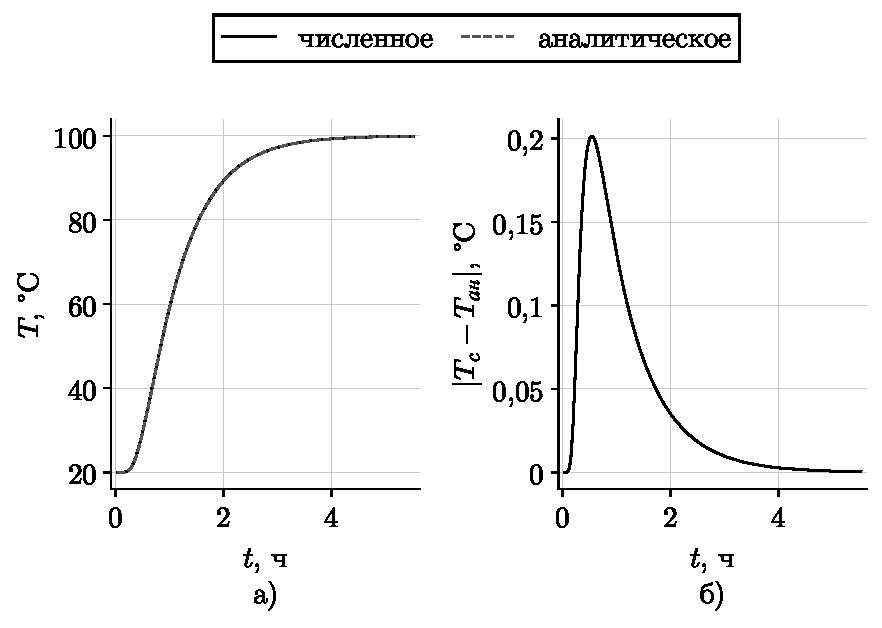
\includegraphics{validation.pdf}
    \caption{Температура в центре куба: численное и аналитическое решения~(а) и абсолютная погрешность численного решения~(б)}
    \label{fig:validation}
\end{figure}

\subsection{Исследование сходимости численного решения при измельчении сетки}

Совпадение с аналитическим решением на одной сетке ещё не доказывает правильность реализации, поскольку ошибка в программе могла бы проявиться только в порядке сходимости. Поэтому расчёт той же задачи был повторён на четырёх сетках, шаг которых последовательно уменьшался вдвое. Шаг по времени при этом выбирался программой автоматически из условия~\eqref{eq:stab}. Погрешность сравнивалась в момент $t = 4000$~с, а численное значение в этот момент находилось линейной интерполяцией между ближайшими шагами по времени. Результаты сравнения приведены в таблице~\ref{tab:conv}.

\begin{table}[ht]
    \centering
    \caption{Погрешность температуры в центре куба при $t = 4000$~с}
    \label{tab:conv}
    \begin{tabular}{|c|c|c|c|c|}
        \hline
        Сетка & $h$, м & $T_c$, °C & $|T_c - T_{\text{ан}}|$, °C & Отношение погрешностей \\
        \hline
        $11^3$ & 0,1000 & 65,383 & 1,0113 & --- \\
        $21^3$ & 0,0500 & 64,626 & 0,2543 & 3,98 \\
        $41^3$ & 0,0250 & 64,435 & 0,0636 & 4,00 \\
        $81^3$ & 0,0125 & 64,387 & 0,0159 & 4,00 \\
        \hline
    \end{tabular}
\end{table}

Аналитическое значение температуры в этот момент равно 64,371~°C. Из таблицы видно, что при каждом уменьшении шага сетки вдвое погрешность уменьшается ровно в четыре раза. Такое поведение означает второй порядок сходимости по пространству, который и должна обеспечивать схема~\eqref{eq:ftcs}. Первый порядок аппроксимации по времени не нарушает эту картину, так как шаг по времени пропорционален $h^2$ и вносимая им ошибка убывает так же быстро.

\subsection{Совпадение результатов при различном числе вычислительных потоков}

Для параллельной программы недостаточно проверить точность одного расчёта, так как ошибки синхронизации проявляются случайно и зависят от числа потоков. Поэтому одна и та же задача с несимметричными граничными условиями на сетке $21^3$ рассчитывалась одним и четырьмя потоками, после чего все файлы результатов сравнивались поэлементно. Значения температуры во всех срезах поля совпали побитно, то есть без какого-либо различия даже в последнем разряде. Такой результат объясняется тем, что каждый узел вычисляется по одной и той же формуле с одними и теми же исходными данными, а от числа потоков зависит только то, какой поток выполняет вычисление.

Аналогичное сравнение было выполнено для исполняемых файлов, собранных для Linux и для Windows. Версия для Windows запускалась в среде совместимости Wine, и её результаты также совпали с результатами версии для Linux побитно, а различие файлов состояло лишь в символах перевода строки. Оба сравнения включены в набор автоматических тестов и выполняются при каждом изменении исходного кода.

\section{Исследование производительности параллельной версии на многоядерном процессоре}

\subsection{Методика проведения замеров времени выполнения расчёта}

Замеры выполнялись на четырёхъядерном процессоре Intel Xeon с тактовой частотой 2,1~ГГц под управлением операционной системы Linux. Расчётный модуль был собран компилятором GCC версии 13.3 с уровнем оптимизации \texttt{-O2}. Рассматривались кубические сетки $50^3$, $100^3$ и $150^3$, содержащие от 125 тысяч до 3,4 миллиона узлов, а число потоков менялось от одного до четырёх.

Чтобы время расчёта на разных сетках было сопоставимым, на каждой сетке выполнялась ровно тысяча шагов по времени, а запись промежуточных результатов была отключена. Каждый расчёт повторялся пять раз, и в качестве результата принималось наименьшее время. Такой выбор исключает случайные задержки, вызванные другими процессами операционной системы, и характеризует возможности самой программы. Ускорение и эффективность вычислялись по формулам~\eqref{eq:speedup}.

\subsection{Ускорение и эффективность для расчётных сеток разного размера}

Измеренное время расчёта приведено в таблице~\ref{tab:bench}. Последовательная версия программы, собранная без поддержки OpenMP, на сетке $100^3$ выполняет расчёт за 2,02~с, то есть практически за то же время, что и параллельная версия на одном потоке. Это означает, что сами директивы OpenMP не создают заметных накладных расходов.

\begin{table}[ht]
    \centering
    \caption{Время расчёта 1000 шагов по времени, с}
    \label{tab:bench}
    \begin{tabular}{|c|c|c|c|c|c|c|}
        \hline
        Сетка & $p = 1$ & $p = 2$ & $p = 3$ & $p = 4$ & $S_4$ & $E_4$ \\
        \hline
        $50^3$  & 0,231 & 0,132 & 0,107 & 0,085 & 2,72 & 0,68 \\
        $100^3$ & 1,879 & 1,010 & 0,737 & 0,548 & 3,43 & 0,86 \\
        $150^3$ & 6,837 & 3,520 & 2,565 & 2,121 & 3,22 & 0,81 \\
        \hline
    \end{tabular}
\end{table}

Зависимость ускорения и эффективности от числа потоков для трёх сеток показана на рисунке~\ref{fig:speedup}. На рисунке~\ref{fig:speedup},~а кривые для сеток $100^3$ и $150^3$ идут вблизи идеальной прямой $S_p = p$ и при четырёх потоках достигают значений 3,43 и 3,22 соответственно. Кривая для сетки $50^3$ заметно отклоняется от идеальной уже при трёх потоках, и итоговое ускорение составляет 2,72. На рисунке~\ref{fig:speedup},~б эта разница видна ещё отчётливее: эффективность для больших сеток при четырёх потоках остаётся на уровне 0,81--0,86, тогда как для малой сетки она снижается до 0,68.

\begin{figure}[ht]
    \centering
    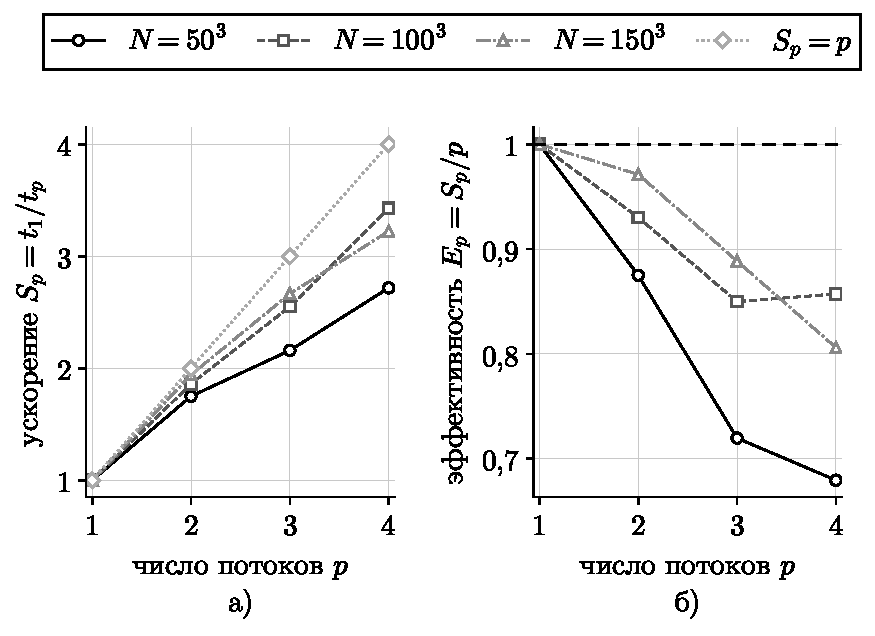
\includegraphics{fig_speedup.pdf}
    \caption{Ускорение~(а) и эффективность~(б) параллельной версии программы в зависимости от числа потоков для сеток разного размера}
    \label{fig:speedup}
\end{figure}

Снижение эффективности на малой сетке объясняется соотношением полезной работы и накладных расходов. На сетке $50^3$ один шаг по времени выполняется за доли миллисекунды, а на каждом шаге программа проходит через четыре параллельные области, в конце каждой из которых потоки синхронизируются. Время синхронизации от размера сетки не зависит, поэтому на малой сетке его доля оказывается значительной. На больших сетках доля синхронизации мала, и основным ограничением становится пропускная способность памяти, о которой говорилось в первой главе. Различие между сетками $100^3$ и $150^3$ находится в пределах разброса повторных замеров, составляющего около 5--10~\%.

\subsection{Влияние последовательной записи результатов на итоговое ускорение}

В рассмотренных замерах запись результатов была отключена, однако в реальной работе программа периодически сохраняет срезы температурного поля для последующей визуализации. Запись в файлы выполняется одним потоком, и для оценки её влияния был проведён отдельный эксперимент на сетке $100^3$. При одной и той же тысяче шагов число записей $M$ менялось от нуля до ста, а время расчёта измерялось на одном и на четырёх потоках. Для сравнения с замерами использовалась простая модель, в которой время записи не уменьшается при увеличении числа потоков, а время вычислений уменьшается так же, как в расчёте без записи.

Результаты эксперимента приведены на рисунке~\ref{fig:io}. На рисунке~\ref{fig:io},~а время расчёта на обоих потоках растёт с увеличением числа записей, причём для одного потока каждая запись добавляет около 17~мс. Поскольку это время одинаково для любого числа потоков, разрыв между кривыми в относительном выражении сокращается. На рисунке~\ref{fig:io},~б видно, что ускорение на четырёх потоках падает с 3,39 при отсутствии записи до 2,16 при двадцати записях и до 1,34 при ста записях.

\begin{figure}[ht]
    \centering
    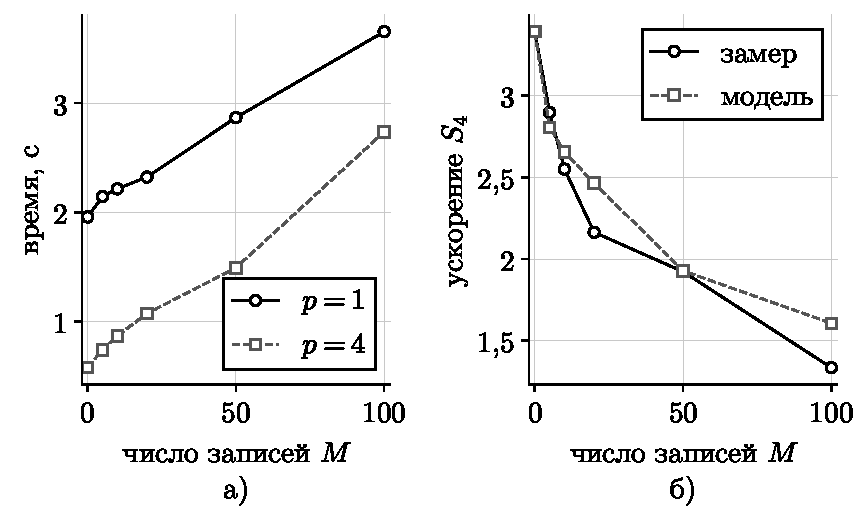
\includegraphics{io.pdf}
    \caption{Время расчёта~(а) и ускорение на четырёх потоках~(б) в зависимости от числа записей результатов на сетке $100^3$}
    \label{fig:io}
\end{figure}

Модельная кривая хорошо описывает замеры при небольшом числе записей, что подтверждает применимость закона Амдала~\eqref{eq:amdahl} к данной программе. При ста записях на запись приходится 0,46 времени последовательного расчёта, и модель предсказывает ускорение не выше 1,6. Фактическое ускорение оказывается ещё ниже модельного, вероятно, из-за того, что во время записи остальные потоки простаивают в ожидании, а данные расчётного массива вытесняются из кэша процессора. Отсюда следует практическая рекомендация: при длительных расчётах интервал записи следует выбирать так, чтобы число сохранённых срезов составляло десятки, а не сотни. Дальнейшее повышение эффективности возможно за счёт выполнения записи в отдельном потоке одновременно с вычислением следующих шагов.
